%% main.tex — 紀要「文化情報学」LaTeX テンプレート 使用例兼説明書
%%
%% このファイルを書き換えて原稿を作ります。
%% 「%」から行末まではコメント（PDF には出ません）。
%% Overleaf では Menu → Compiler を「LuaLaTeX」にしてください。

%% ---------------------------------------------------------------
%% 種別: [ ] の中を書き換える
%%   paper（研究論文）/ note（研究ノート）/ material（資料紹介）/ review（書評）
%%   英語論文は [paper,english] のように english を加える
%% ---------------------------------------------------------------
\documentclass[paper]{bunkajoho}

%% 文献データのファイル（このファイルと同じ場所に置く）
\addbibresource{sample.bib}

%% 表題・副題・著者名
\title{紀要「文化情報学」LaTeX テンプレートの使い方}
\subtitle{執筆要項に基づくクラスファイルと文献スタイル}   % 副題がなければこの行を消す
\author{同志社 太郎・文化 花子}                           % 複数の著者は「・」で区切る

%% 要旨（和文・英文いずれでもよい）
\begin{abstract}
本稿は、同志社大学文化情報学会紀要『文化情報学』の執筆要項（2022 年 12 月 7 日改訂）に基づいて作成した LaTeX テンプレートの使い方を示すものである。
本文そのものが使用例となっており、タイトルページの構成、節番号、図表、数式、脚注、参照文献の書き方を順に説明する。
このファイル（main.tex）を開き、PDF と見比べながら書き換えていけば原稿になる。
\end{abstract}

\begin{document}
\maketitle   % ここにタイトル部（種別・表題・著者名・要旨）が出る

%% ---------------------------------------------------------------
%% 本文
%% ---------------------------------------------------------------
\section{はじめに}

執筆要項では、掲載論文は LaTeX または Microsoft Word で作成し、編集委員会が用意したスタイルファイルを用いることとされている。
本テンプレートはその LaTeX 版の叩き台である。
この PDF は main.tex から作られており、main.tex を書き換えることで原稿を作成できる。

ファイルの先頭にある次の行の \verb|paper| を書き換えると、第 1 ページ左上の種別ラベルが変わる。
\begin{verbatim}
\documentclass[paper]{bunkajoho}
\end{verbatim}
\verb|note| は研究ノート、\verb|material| は資料紹介、\verb|review| は書評になる。
表題・副題・著者名は、それぞれ \verb|\title{...}|、\verb|\subtitle{...}|、\verb|\author{...}| の中に書く。
要旨は \verb|abstract| 環境の中に書く。

第 1 ページには、要項 4. のとおり、タイトル・種別・著者名・アブストラクトが置かれる。
ページ番号は事務局が付けるため、投稿原稿には付けない。

段落を改めるには、空行を 1 行入れる。
ソースの中で改行しただけでは段落は変わらない。

\section{本文の書き方}

\subsection{節と項}

本文は節から構成し、各節には 1、2.3、3.4.2 のように番号を付ける（要項 5.）。
LaTeX では \verb|\section{見出し}|（節）、\verb|\subsection{見出し}|（項）、
\verb|\subsubsection{見出し}|（目）と書くと、番号は自動で付く。

\subsubsection{表記上の注意}

日本語で執筆する場合、句読点は「、」と「。」を用いる。
専門用語は原則として日本語で表記し、必要なら初出時のみ欧文を丸括弧内に併記する。
たとえば「アフォーダンス（affordance）」のように書く。
略語は初出時に正式名を記し、続けて丸括弧内に略語を示す。
たとえば「大規模言語モデル（Large Language Model; LLM）」とする。

\subsubsection{特別な意味をもつ文字}

\verb|% $ & # _ { } ~ ^ \| の各文字は LaTeX の命令に使われるため、そのままでは本文に出ない。
本文に「\%」や「\&」を出すには、\verb|\%|、\verb|\&| のように前に \verb|\| を付ける。
全角の「％」「＆」はそのまま書いてよい。

\subsection{数式}

数式は別行に記し、末尾に通し番号を付ける。
別行の数式は \verb|equation| 環境の中に書く。
\begin{equation}
  H(X) = -\sum_{i=1}^{n} p(x_i) \log_2 p(x_i)
  \label{eq:entropy}
\end{equation}
本文中に埋め込む場合には、\verb|$a/b$| のように \verb|$| で囲み、
$a/b$、$\exp(x/y)$、$\delta x/\delta t$ のような記法を用いる。

式に \verb|\label{eq:mi}| のように名前を付けておくと、
\verb|式 \eqref{eq:mi}| と書いて「式 \eqref{eq:mi}」のように番号を参照できる。
式を追加・削除しても番号は自動で付け直される。
\begin{equation}
  I(X;Y) = H(X) - H(X \mid Y)
  \label{eq:mi}
\end{equation}

\subsection{注}

注はなるべく用いない\footnote{止むを得ず使用する場合は、このように \texttt{\textbackslash footnote\{...\}} で書く。刷り上がりではすべて脚注となる。}。

\section{図表}

図表には「図 1」「表 1」のように通し番号を付け、キャプションは原則として日本語で書く（要項 6.）。
図~\ref{fig:example} と表~\ref{tab:example} に例を示す。
図表にも \verb|\label{...}| で名前を付け、本文では \verb|図~\ref{fig:example}| のように参照する。
図表は段の上端か下端に自動で配置されるため、ソースに書いた位置とずれることがある。

査読用原稿では図表を本文中に埋め込んで提出し、採択後の最終原稿では図の相当部分を空白にして充分な解像度のデータを別途提出する（要項 4.）。
他の文献から転載する場合は、著作権者の了解を得たうえで出典を明記する。

%% 図: 画像ファイル（PNG, JPEG, PDF）をこのファイルと同じ場所に置き、ファイル名を書く。
%%   width=0.9\linewidth は「段の幅の 90%」
\begin{figure}[tb]
  \centering
  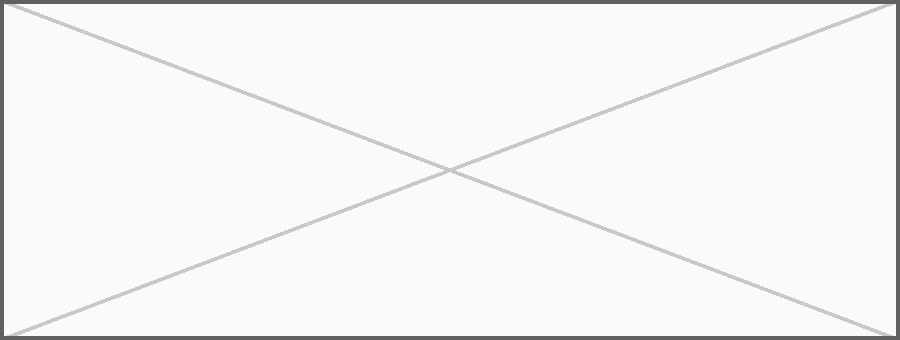
\includegraphics[width=0.9\linewidth]{figure1.png}
  \caption{図の例}
  \label{fig:example}
\end{figure}

%% 表: {lrr} は各列の揃え（l 左, c 中央, r 右）。列は & で区切り、行末に \\ を書く。
%%   キャプションは表の上に置く。
\begin{table}[tb]
  \centering
  \caption{表の例}
  \label{tab:example}
  \begin{tabular}{lrr}
    \toprule
    項目 & 度数 & 割合（\%） \\
    \midrule
    研究論文 & 12 & 60.0 \\
    研究ノート & 5 & 25.0 \\
    書評 & 3 & 15.0 \\
    \bottomrule
  \end{tabular}
\end{table}

2 段にまたがる大きな図表は、\verb|figure| / \verb|table| の代わりに
\verb|figure*| / \verb|table*| を使う（表~\ref{tab:cite} がその例）。
この場合、図の幅 \verb|\linewidth| は 2 段分の幅になる。

\section{参照文献}

\subsection{本文中での引用}

本文中で文献を参照する際は、著者の姓の後に発表年を西暦で記す（要項 7.）。
LaTeX では \verb|\citet{キー}| または \verb|\citep{キー}| と書くと、
著者名と発表年が要項の形式で自動的に出力される。
キーは文献データ（sample.bib）で各文献に付けた名前である。
表~\ref{tab:cite} に要項の例と対応する書き方を示す。

\begin{table*}[tb]
  \centering
  \caption{引用の書き方と出力}
  \label{tab:cite}
  \footnotesize
  \begin{tabular}{ll}
    \toprule
    書き方 & 出力 \\
    \midrule
    \verb|\citet{gibson1979}| & \citet{gibson1979} \\
    \verb|\citep{saeki1990}| & \citep{saeki1990} \\
    \verb|\citet[123]{haugeland1987}| & \citet[123]{haugeland1987} \\
    \verb|Simon \citep*{simon1973,simon1981}| & Simon \citep*{simon1973,simon1981} \\
    \verb|\citep{simon1973,simon1981}| & \citep{simon1973,simon1981} \\
    \verb|\citet{cohen1990a}| & \citet{cohen1990a} \\
    \verb|\citep{cohen1990a,cohen1990b}| & \citep{cohen1990a,cohen1990b} \\
    \verb|\citep{anzai1992,joshi1981,minsky1975,minsky1986}| & \citep{anzai1992,joshi1981,minsky1975,minsky1986} \\
    \bottomrule
  \end{tabular}
\end{table*}

文章の一部として読む場合は \citet{gibson1979} によれば\ldots\ldots のように \verb|\citet| を使い、
そうでない場合は\ldots\ldots が提唱されている\citep{saeki1990}のように \verb|\citep| を使う。
ページを示すには \verb|\citet[123]{haugeland1987}| のように \verb|[ ]| 内にページ番号を書く。

\subsection{文献データの書き方}

引用する文献は、sample.bib のような bib ファイルにまとめて書く。
たとえば雑誌論文は次のように書く。

\begin{small}
\begin{verbatim}
@article{miller1956,
  author       = {Miller, G. A.},
  year         = {1956},
  title        = {The Magical Number ...},
  journaltitle = {Psychological Review},
  volume       = {63},
  number       = {1},
  pages        = {81-97},
}
\end{verbatim}
\end{small}

1 行目の \verb|miller1956| がキーである。
和文文献には \verb|langid = {japanese}| を付け、著者は \verb|{佐伯, 胖 and 佐々木, 正人}| のように「姓, 名」を \verb|and| で区切って書く。
欧文文献と混ぜて正しい位置に並ぶよう、\verb|sortname| にローマ字読みを書き、キーもローマ字（姓＋年）にする。
書籍・論文集・翻訳書などの書き方は sample.bib の例を参照のこと。

\subsection{文献リスト}

文献リストは、\verb|\printbibliography| と書いた位置に「文献」という見出しのもとに出力される。
本文中で引用した文献だけが載り、欧文と和文を区別せず、第 1 著者の姓のアルファベット順に並び、番号は付かない。
以下は要項に挙げられた例をすべて引用したものである：
\citet{miller1956}、\citet{cohen1985}、Minsky \citep*{minsky1986,minsky1986b}、\citet{saeki1990}、
\citet{minsky1975}、\citet{perrault1990b}、\citet{rosenschein1987}、\citet{devins1981}。

\section{おわりに}

本テンプレートは非公式の叩き台である。
判型・字詰め・フォントサイズなどは、刊行された論文の組版に合わせている。

%% 謝辞（不要なら消す）
\begin{acknowledgments}
謝辞は本文の後、文献の前に置く。
謝辞は \verb|acknowledgments| 環境の中に書く。
\end{acknowledgments}

%% 文献リスト
\printbibliography

%% 付録（不要なら \appendix 以下を消す）
\appendix

\section{付録の例}

付録は文献の後に置く。
\verb|\appendix| の後の \verb|\section| は「付録 A」のような番号になる。

\end{document}
